\documentclass{acm_proc_article-sp}
\usepackage[utf8]{inputenc}

\renewcommand{\paragraph}[1]{\vskip 6pt\noindent\textbf{#1 }}
\usepackage{hyperref}
\usepackage{graphicx}
\usepackage{url}

\providecommand{\tightlist}{%
  \setlength{\itemsep}{0pt}\setlength{\parskip}{0pt}}

\title{R Shiny Investigative Tool into GASTech Personnel Disappearance}


% Add imagehandling
\usepackage{graphicx}
% Redefine \includegraphics so that, unless explicit options are
% given, the image width will not exceed the width of the page.
% Images get their normal width if they fit onto the page, but
% are scaled down if they would overflow the margins.
\makeatletter
\def\ScaleIfNeeded{%
  \ifdim\Gin@nat@width>\linewidth
    \linewidth
  \else
    \Gin@nat@width
  \fi
}
\makeatother
\let\Oldincludegraphics\includegraphics
{%
 \catcode`\@=11\relax%
 \gdef\includegraphics{\@ifnextchar[{\Oldincludegraphics}{\Oldincludegraphics[width=\ScaleIfNeeded]}}%
}%

\numberofauthors{2}
\author{
\alignauthor Aryah Umralkar Chopra \\
        \affaddr{School of Computing and Information Systems, Singapore
Management University}\\
       \email{\href{mailto:aryahc.2020@mitb.smu.edu.sg}{\nolinkurl{aryahc.2020@mitb.smu.edu.sg}}}
\and \alignauthor Rhoda Tong Min Ting \\
        \affaddr{School of Computing and Information Systems, Singapore
Management University}\\
       \email{\href{mailto:rhoda.tong.2020@mitb.smu.edu.sg}{\nolinkurl{rhoda.tong.2020@mitb.smu.edu.sg}}}
\and \alignauthor Davmes Tan Chee Seng \\
        \affaddr{School of Computing and Information Systems, Singapore
Management University}\\
       \email{\href{mailto:davmes.tan.2020@mitb.smu.edu.sg}{\nolinkurl{davmes.tan.2020@mitb.smu.edu.sg}}}
\and }

\date{}

%Remove copyright shit
\permission{}
\conferenceinfo{} {}
\CopyrightYear{}
\crdata{}

% Pandoc syntax highlighting

% Pandoc citation processing


\begin{document}
\maketitle

\begin{abstract}
A fictitious scenario was created as part of VAST Challenge 2021. A
group of staff members from GASTech, an oil and gas company situated on
an island known as Abila on Kronos, had gone missing mysteriously. A
group known as Protectors of Kronos (POK) was the prime suspect into the
disappearance. A series of unprocessed data were made available to the
law enforcement agencies to investigate on. The data were split across
three mini challenges, which our team had undertaken Mini Challenge 1
and 2.

Mini Challenge 1 consists of email correspondences, employee records and
resumes, historical documents and news articles. The ojective of this
mini challenge is to identify the complex relationships among the people
and organisations, and possibly infer the disappearance of GASTech to
any individuals/group who might be involved. Mini Challenge 2 consists
of gps tracking, transaction and loyalty card records, together with car
assignment records - linked to the gps tracking data. The objective of
this mini challenge is to discover anomalies and suspicious activites
that may require additional investigating.

The objective of this research paper is to share on the methods and
models used to develop an online investigative tool where a law
enforcement at Kronos and Tethys could use, to piece the raw data into
useable information and evidences.
\end{abstract}

\hypertarget{introduction}{%
\section{Introduction}\label{introduction}}

A fictitious scenario was created as part of VAST Challenge 2021. A
group of staff members from GASTech, an oil and gas company situated on
an island known as Abila on Kronos, had gone missing mysteriously. A
group known as Protectors of Kronos (POK) was the prime suspect into the
disappearance. While Mini Challenge 1 and 2 provided a set of raw data
that allow investigators to establish and identify complex relationships
among the people and organisations, discover anomalies and suspicious
activities, such investigative work may require humongous man hours and
effort, without data analytics and visualisation.

We would be using Shiny R to develop an online investigative tool to aid
in the analysis into the disappearance of GASTech Personnel, allowing
investigators to explore information and inferential statistics derived
from the unprocessed data available.

\hypertarget{motivation}{%
\section{Motivation}\label{motivation}}

The motivation of this project would be two-fold. First, the data
presented to the investigators were raw and unprocessed, and to link and
derive insights from these data would require tremendous man hours and
effort. Second, while insights could be derived and useful information
could be formed, there would be a need to present the information in a
visually appealing format to facilitate information dissemination and to
allow quick collective appreciation of events among the investigators.

To this end, we would be looking to develop a R Shiny app based on three
principles: (a) informative; (b) intuitive and; (c) interactive. Our 3Is
principles would have the data undergoing baseline cleaning, making them
into suitable formats for subsequent processing for information
delivery. The user-interface would be made intuitive so that the
investigator would be able to use the application without much
references to our user guide. The online investigative tool would also
be interactive, such that the investigator would be able to provide
varied inputs into the formation towards the final visualisation report.

The R Shiny app would comprise of two main modules: (a) Exploratory Data
Analysis allowing investigators to draw information such as transaction
records, employee records, email correspondences and such; (b)
Inferential Statistics allowing investigators to infer relationship
linkages among user-selected employees, possible coded words within
email correspondences within an identified group of personnel, their
movements towards identified locations and possible anomalies at the
locations and transaction analysis using both credit card and loyalty
card data.

\hypertarget{review-and-critic-of-past-works}{%
\section{Review and Critic of Past
Works}\label{review-and-critic-of-past-works}}

Taking reference on a submission by students from International
Institute of Information Technology Hyderabad, they had derived an
interface that uses geotools to show the paths of the cars, moving at a
particular time or date. While it was a useful tool to visualise the
movement of the vehicles, it was unable to plot the locations where the
vehicles may had visited. This would be addressed in one of our module.

While credit card data and loyalty card data were provided for, to the
investigators, there are no direct linkages between both set of data,
except for the locations and price of item. The timestamp for both data
are recorded differently with the credit card indicating the time of
transaction while loyalty data indicating date of transactions only.
Reviewing past work from members of University of Calgary, they
attempted Parallel Coordinates plot by linking the locations, timestamp,
price and employees, to establish possible linkages among the four
variables. Inspired by their work and the sharing from Prof Kam on using
Parallel Coordinates Plot on R, we would attempt to create parallel
plots and allow the investigators to decide the variables that they are
keen to establish linkages with.

\hypertarget{design-frame}{%
\section{Design Frame}\label{design-frame}}

Our R Shiny Investigative Tool's design would be based on our 3Is
principle.

\emph{Informative} - A series of informative modules would be made
available under the Exploratory Data Analysis (EDA) tab, comprising of:
(a) Locations Exploration; (b) Transactions Exploration; (c) Cards
Exploration; (d) GASTech Employees Information; and (e) Email
Correspondences. Details of each modules would be covered under the
sub-sections later.

\emph{Intuitive} - The entire UI design would be simple and intuitive,
allowing investigators to use it without frequent references to our user
guide. This would be done by ensuring that appropriate input methods
were used and that the UI would be kept as clean and simple as possible.

\emph{Interactive} - The respective modules would require specific
inputs from the investigators before a representative visualisation
could be produced. It would be made interactive such that the
investigators would have the flexibility to select various variables or
inputs to create the desired visualisation. Similarly, the investigators
would have the option to save the produced visualisation separately.

\hypertarget{exploratory-data-analysis}{%
\section{Exploratory Data Analysis}\label{exploratory-data-analysis}}

\hypertarget{locations---for-exploration}{%
\subsection{Locations - For
Exploration!}\label{locations---for-exploration}}

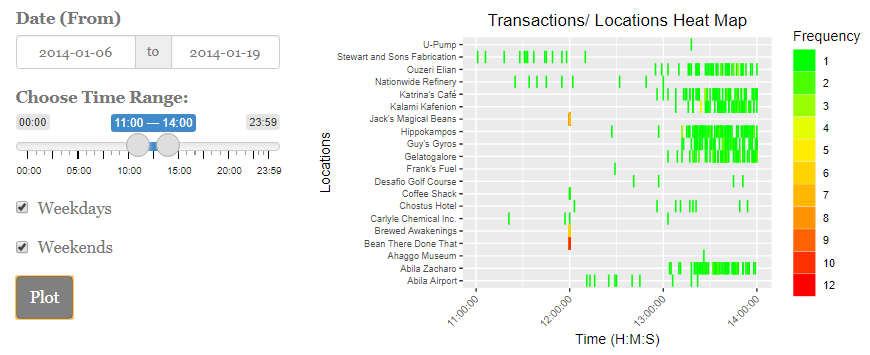
\includegraphics{img/Locations.PNG}

The intention of this module would be to allow the investigators to
explore the popularity of the locations through the analysis of
transaction records. It would be conducted in a manner by aggregating
the transaction records based on the time of transactions. The
transaction counts would be plotted against the aggregated time of
transactions and locations using a heatmap to infer the peak periods for
the locations. The selected records would be filtered based on the range
of date inputs, time range of transactions, with the ability to toggle
between weekdays, weekends or both.

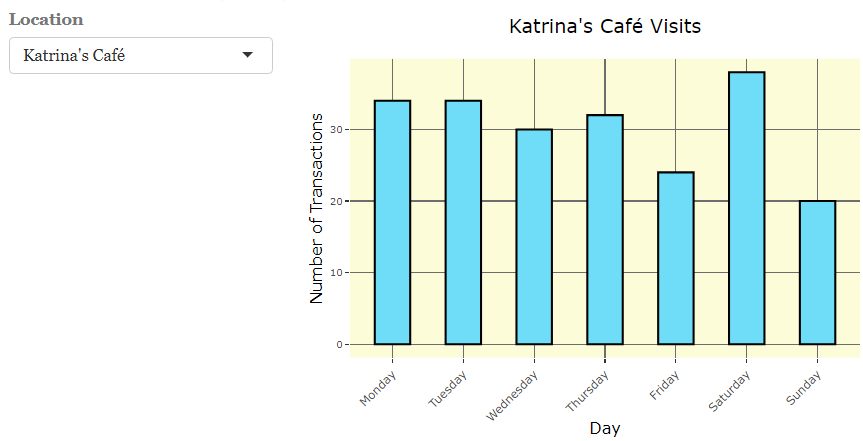
\includegraphics{img/Locations2.PNG}

The function of this module would be to identify the operating days of
the locations through the analysis of credit card transactions, through
the aggregation of records based on the day of transactions. The output
of this visualisation would suggest the days where the locations would
be having transactions, thus inferring their operating days of the week.

\hypertarget{transactions---for-exploration}{%
\subsection{Transactions - For
Exploration!}\label{transactions---for-exploration}}

The intention of this module would be to allow investigators to explore
all credit card and loyalty card transactional records at each location.
The type of visualization chosen enables the investigators to see the
linkages between all variables in one view.

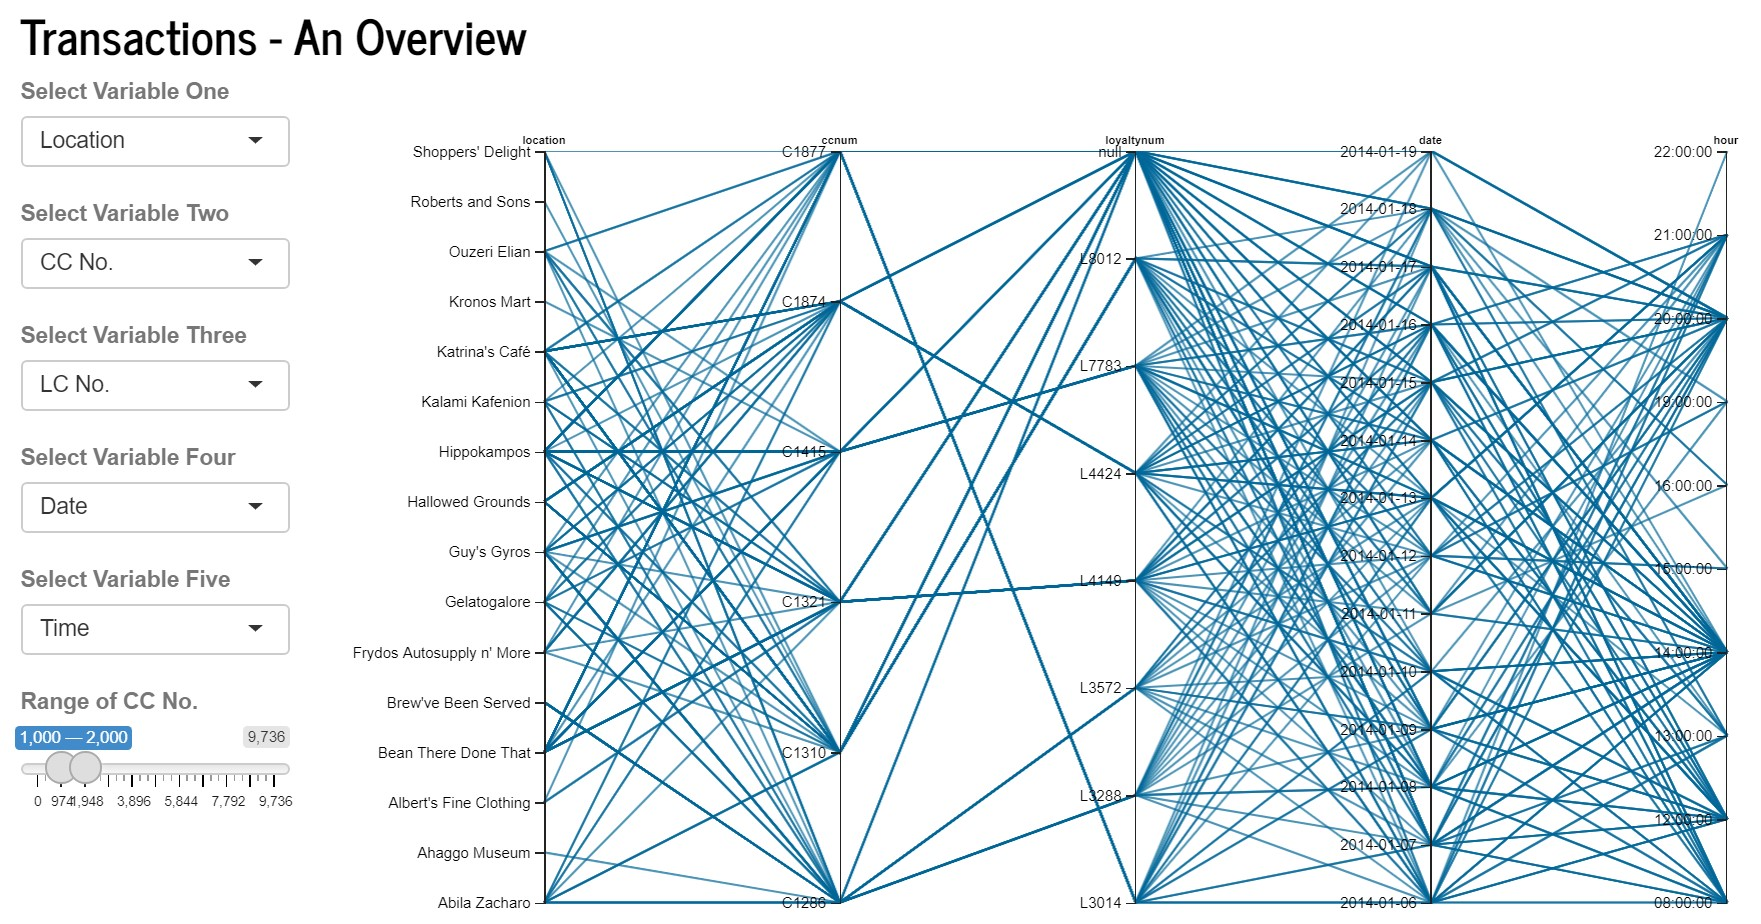
\includegraphics{img/P01Para.jpg}

The plot has multiple functions which would allow the investigator to
customize his/her view and get more insights, such as (1) Variables to
be included can be selected, (2) Variables can be reordered, (3) Range
of Credit Card Numbers to display records for can be selected, (4)
Specific ranges of each variable can be selected so that only associated
links would be shown, (5) Selected ranges can be glided along the axis
to see how the connections change dynamically. These customizations and
flexibilities are important so that the user can zoom in and out on
selected areas of focus, especially when exploring raw data sets. If a
certain value, say for a specific credit card number, appears in
multiple observations, its associations would be clearly displayed in
the form of the series of lines.

\hypertarget{individual-card-transactions}{%
\subsection{Individual Card
Transactions}\label{individual-card-transactions}}

This module allows the investigator to visualize the transactions made
by individual cards for a more in-depth exploration. The page allows the
investigator to select two different cards to be displayed, akin to a
workspace for comparison between cards. This is essentially a deep-dive
compared to the parallel coordinate plot, which gives an overview.

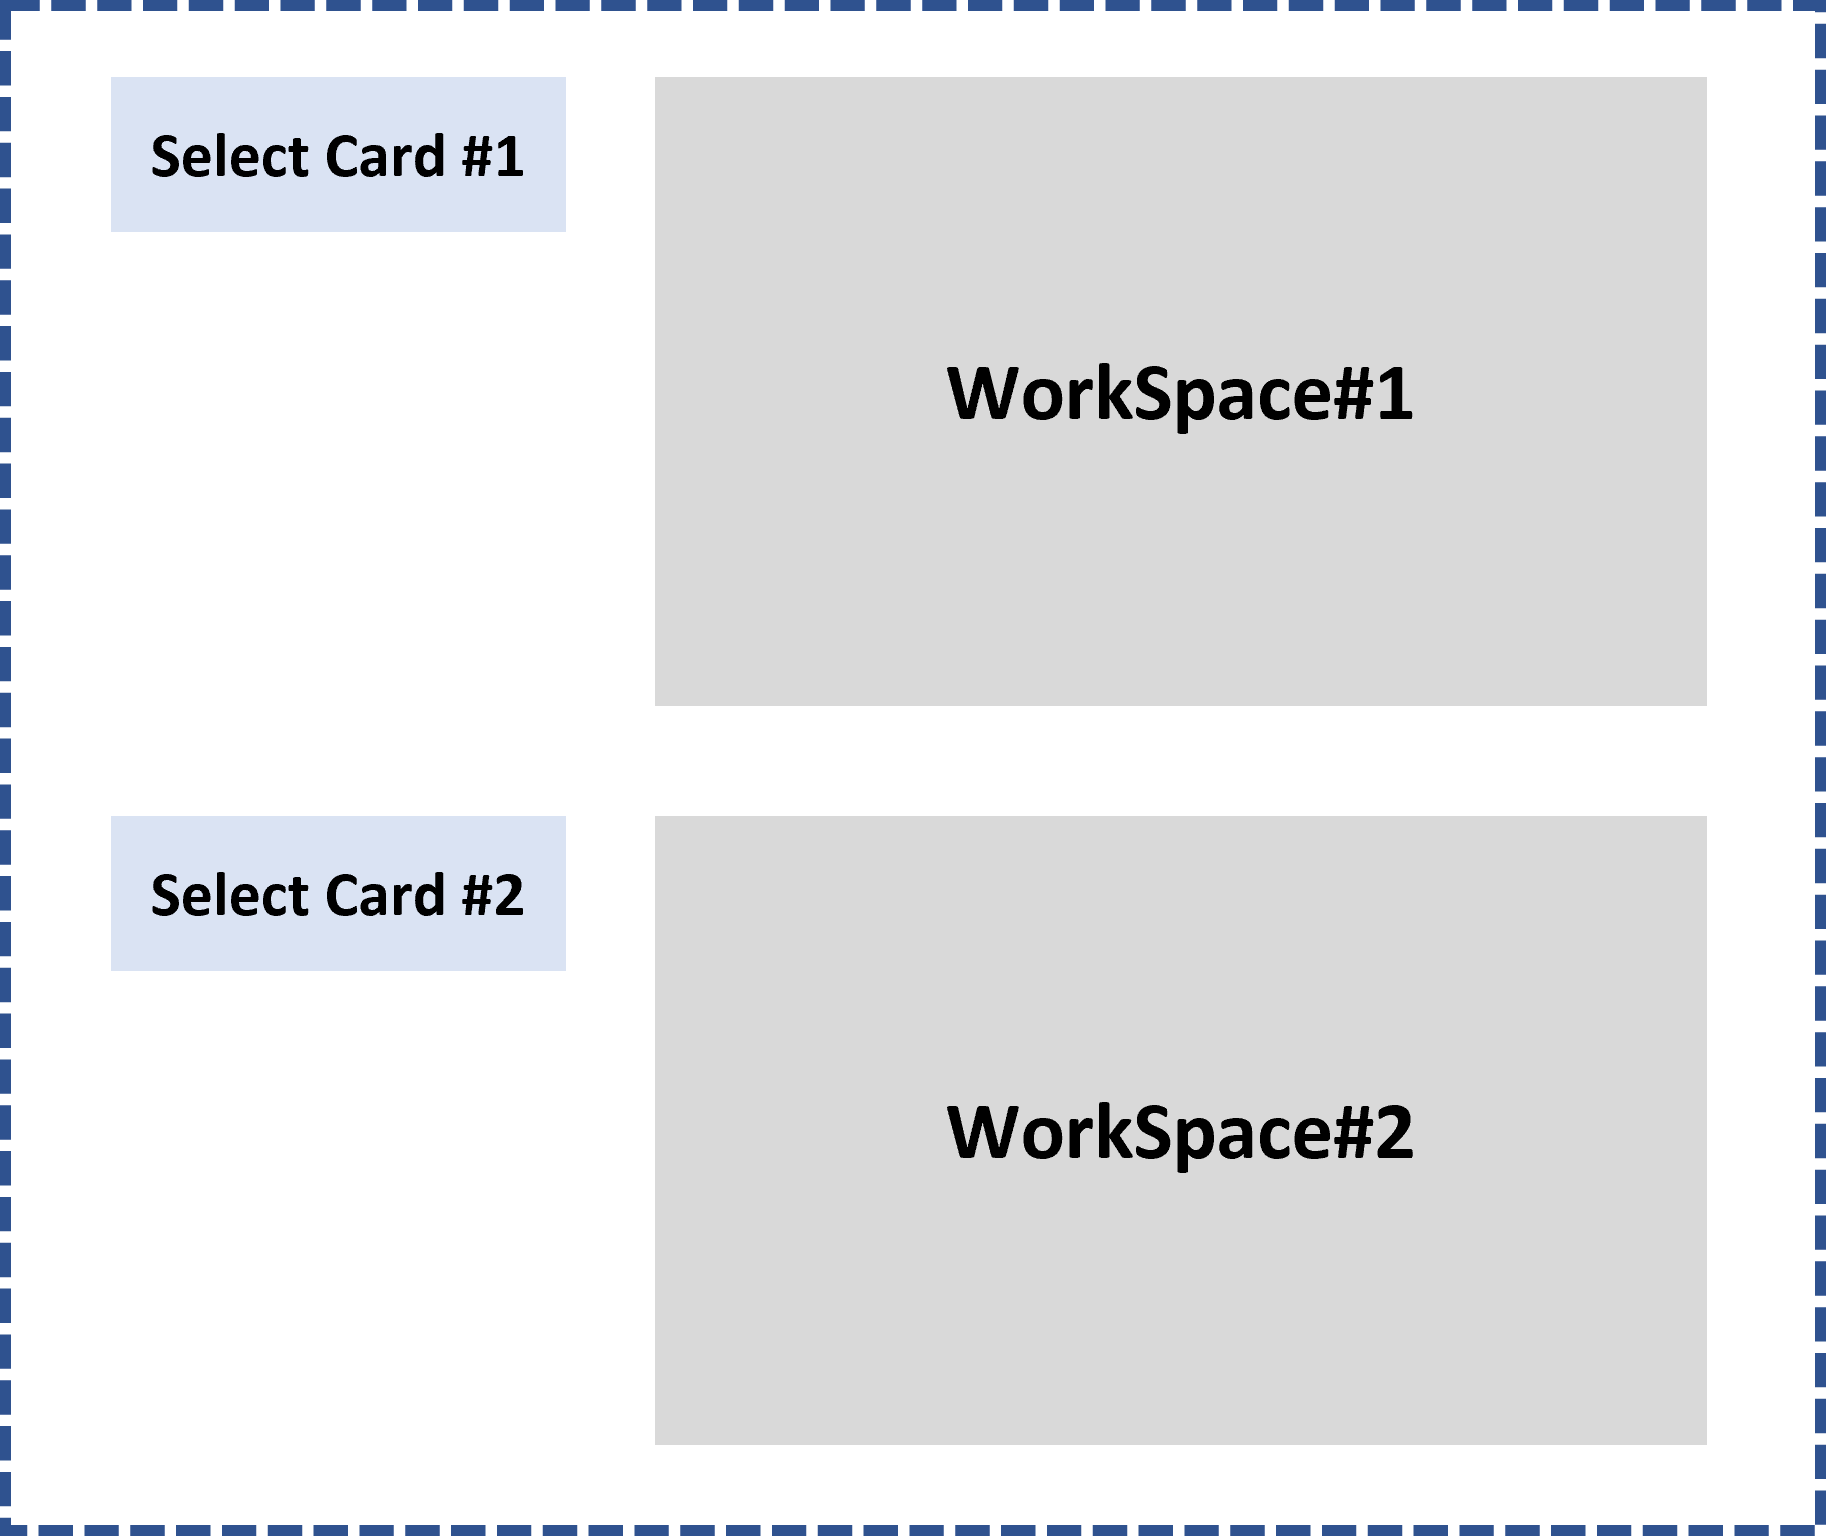
\includegraphics{img/P06WorkSpace.png} The investigator could select the
card type, credit card or loyalty card. If credit card is selected, an
additional field would appear to allow selection of type of fill for the
tiles.

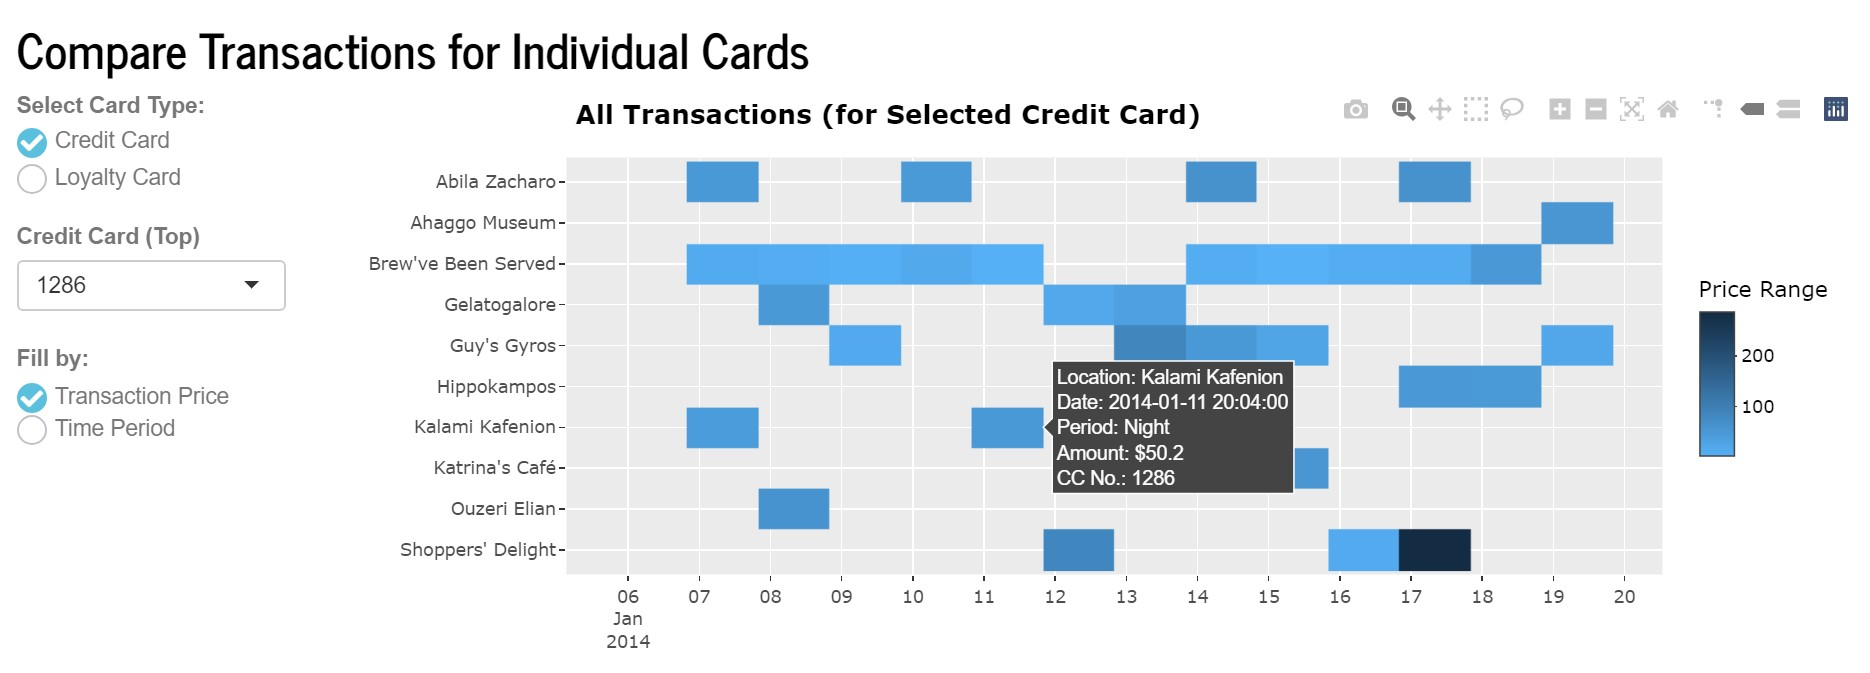
\includegraphics{img/P02SpecCard.jpg}

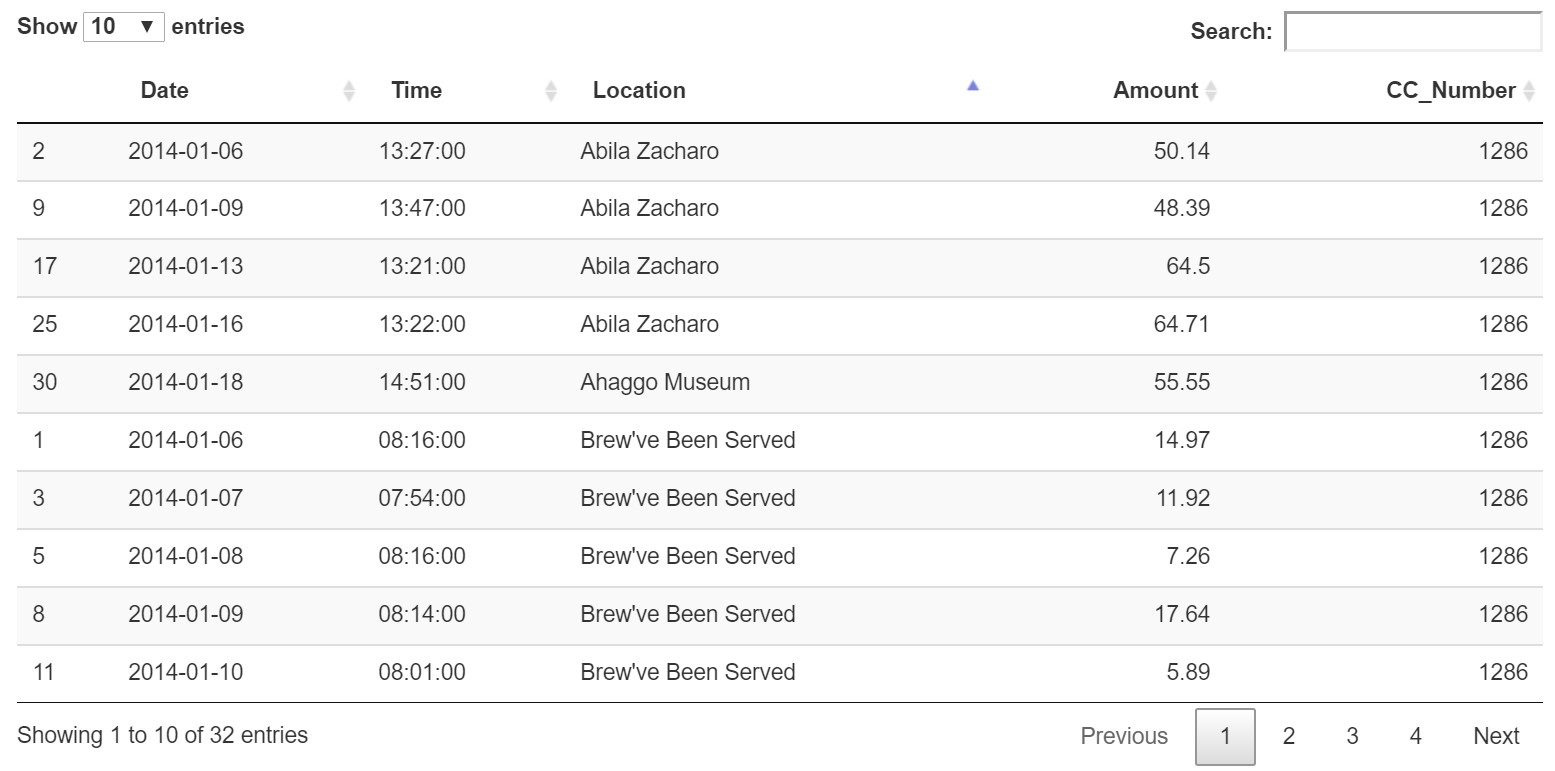
\includegraphics{img/P05SpecCardTable.jpg}

Location is plotted against each day. If there was a transaction at the
location for that day, a tile would appear. For this module, the tile
plot is chosen as its uniform tiles allow a straightforward view of
whether transactions were made consecutively for each day, or on
separate days. The color intensity of the tile would give an indication
of the magnitude of the transaction amount - the darker the intensity,
the higher the amount. Hovering over each tile would display a tooltip
indicating the details of that particular transaction. A data table for
the selected card would also appear below the tile plot to list down all
observations, it can be sorted and filtered, to allow for the
investigator's further exploration.

\hypertarget{employees-of-gastech}{%
\subsection{Employees of GasTech}\label{employees-of-gastech}}

Duis nec purus sed neque porttitor tincidunt vitae quis augue. Donec
porttitor aliquam ante, nec convallis nisl ornare eu. Morbi ut purus et
justo commodo dignissim et nec nisl. Donec imperdiet tellus dolor, vel
dignissim risus venenatis eu. Aliquam tempor imperdiet massa, nec
fermentum tellus sollicitudin vulputate. Integer posuere porttitor
pharetra. Praesent vehicula elementum diam a suscipit. Morbi viverra
velit eget placerat pellentesque. Nunc congue augue non nisi ultrices
tempor.

\hypertarget{email-correspondence}{%
\subsection{Email Correspondence}\label{email-correspondence}}

Duis nec purus sed neque porttitor tincidunt vitae quis augue. Donec
porttitor aliquam ante, nec convallis nisl ornare eu. Morbi ut purus et
justo commodo dignissim et nec nisl. Donec imperdiet tellus dolor, vel
dignissim risus venenatis eu. Aliquam tempor imperdiet massa, nec
fermentum tellus sollicitudin vulputate. Integer posuere porttitor
pharetra. Praesent vehicula elementum diam a suscipit. Morbi viverra
velit eget placerat pellentesque. Nunc congue augue non nisi ultrices
tempor.

\hypertarget{inferential-statistics}{%
\section{Inferential Statistics}\label{inferential-statistics}}

\hypertarget{email-network-analysis}{%
\subsection{Email Network Analysis}\label{email-network-analysis}}

Duis nec purus sed neque porttitor tincidunt vitae quis augue. Donec
porttitor aliquam ante, nec convallis nisl ornare eu. Morbi ut purus et
justo commodo dignissim et nec nisl. Donec imperdiet tellus dolor, vel
dignissim risus venenatis eu. Aliquam tempor imperdiet massa, nec
fermentum tellus sollicitudin vulputate. Integer posuere porttitor
pharetra. Praesent vehicula elementum diam a suscipit. Morbi viverra
velit eget placerat pellentesque. Nunc congue augue non nisi ultrices
tempor.

\hypertarget{networks}{%
\subsection{Networks}\label{networks}}

Duis nec purus sed neque porttitor tincidunt vitae quis augue. Donec
porttitor aliquam ante, nec convallis nisl ornare eu. Morbi ut purus et
justo commodo dignissim et nec nisl. Donec imperdiet tellus dolor, vel
dignissim risus venenatis eu. Aliquam tempor imperdiet massa, nec
fermentum tellus sollicitudin vulputate. Integer posuere porttitor
pharetra. Praesent vehicula elementum diam a suscipit. Morbi viverra
velit eget placerat pellentesque. Nunc congue augue non nisi ultrices
tempor.

\hypertarget{employee-movement-plot}{%
\subsection{Employee Movement Plot}\label{employee-movement-plot}}

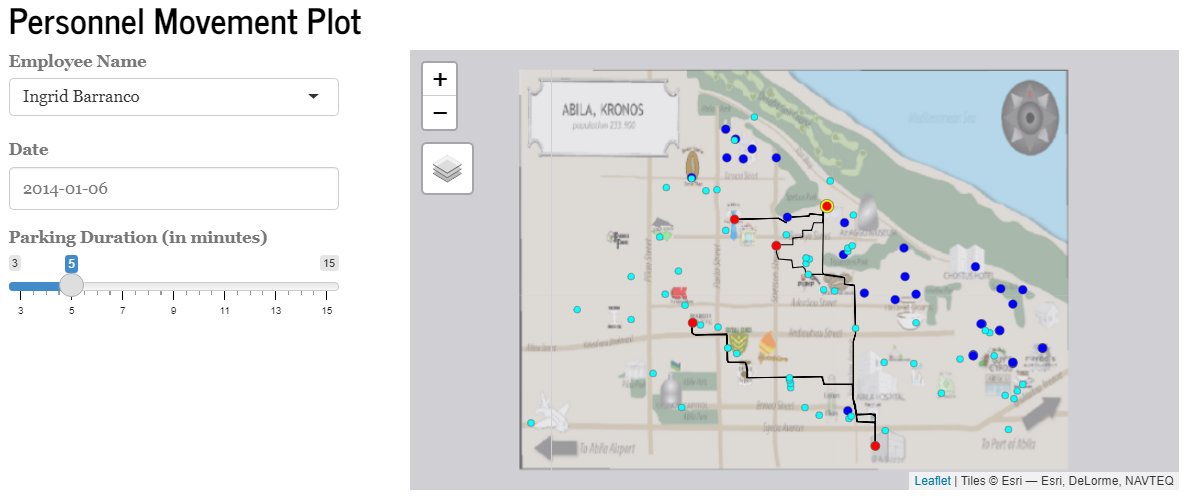
\includegraphics{img/Movement.PNG}

The data preparation for this module would be to identify
Points-of-Interests (POI), using the gps records. Since the recording of
gps would only occur while the vehicle is in motion, whenever there is a
time interval (3g: 3 minutes), would be a good assumption that the
vehicle is in parking mode, thus indicating it as a POI. The time
interval may be adjusted based on the investigators' tolerance between 3
and 15 minutes. The POIs would be differentiated between homes of
employees and other locations, thus allowing tmap to plot the route
taken, and the stops taken.

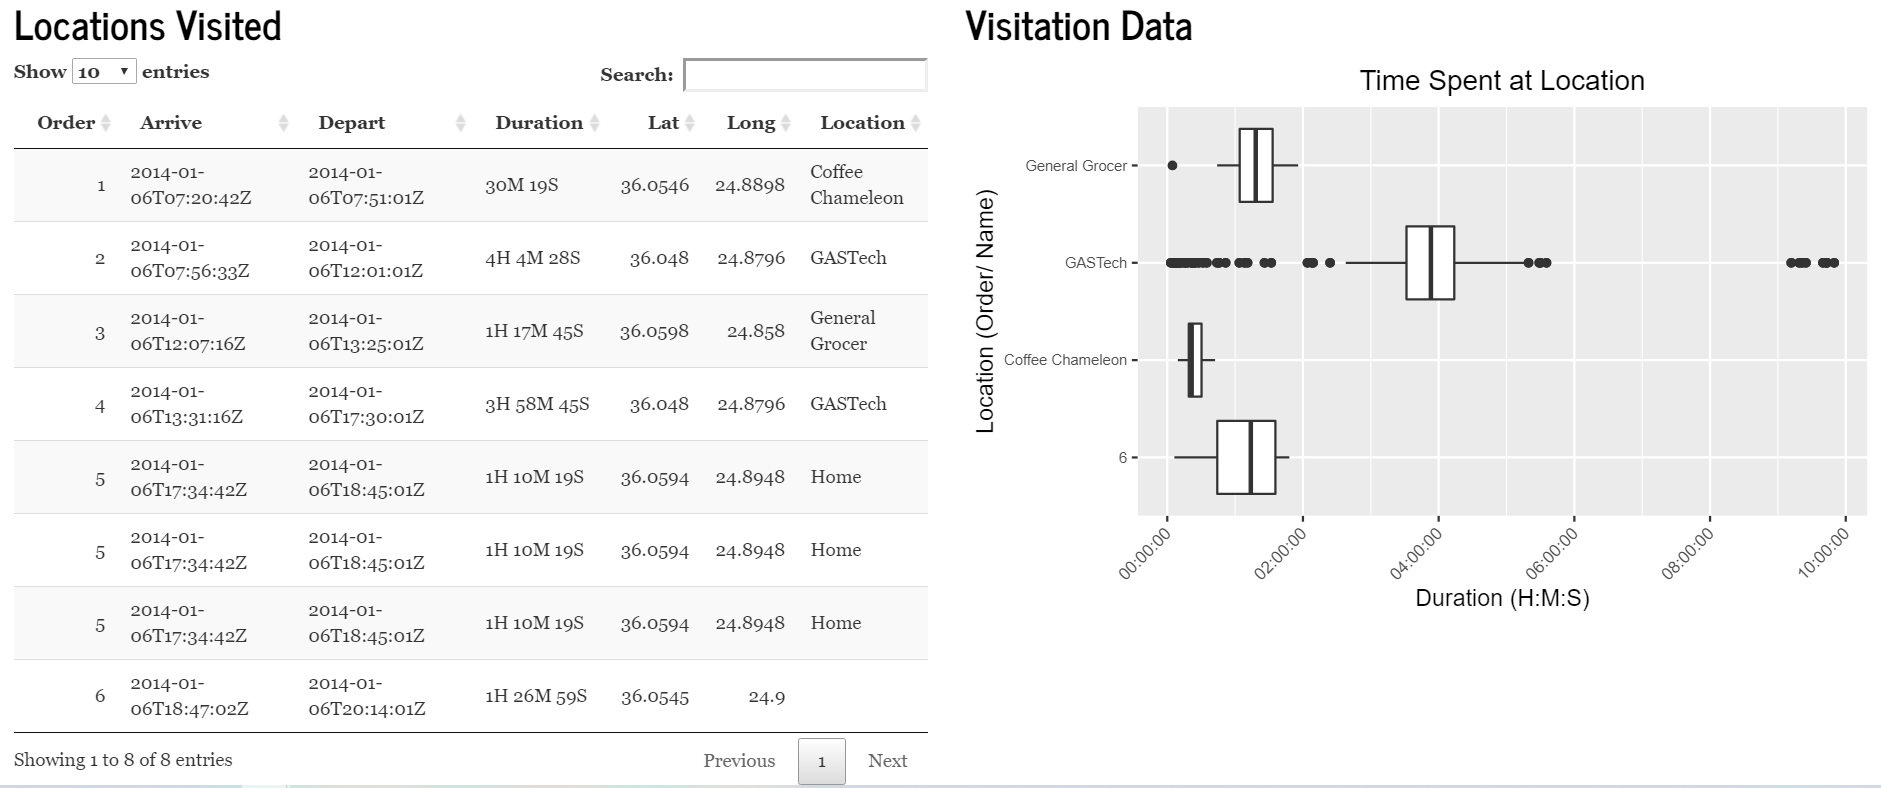
\includegraphics{img/Movement2.PNG}

The sub-module would be an extension where the selected gps plot would
be sequenced based on the time of activity, and further identified based
on marked locations such as their homes, GASTech or prominent locations
that were named prior. The subsequent box plot would be an analysis of
the duration of stop, by visitors, to the locations.

\hypertarget{transaction-amount-analysis}{%
\subsection{Transaction Amount
Analysis}\label{transaction-amount-analysis}}

This module provides statistical analysis on the transactions made at
each location, by each card type. The distribution of the spread of the
transaction amounts is shown by boxplots. Outliers are highlighted in
red to gain the investigator's attention.

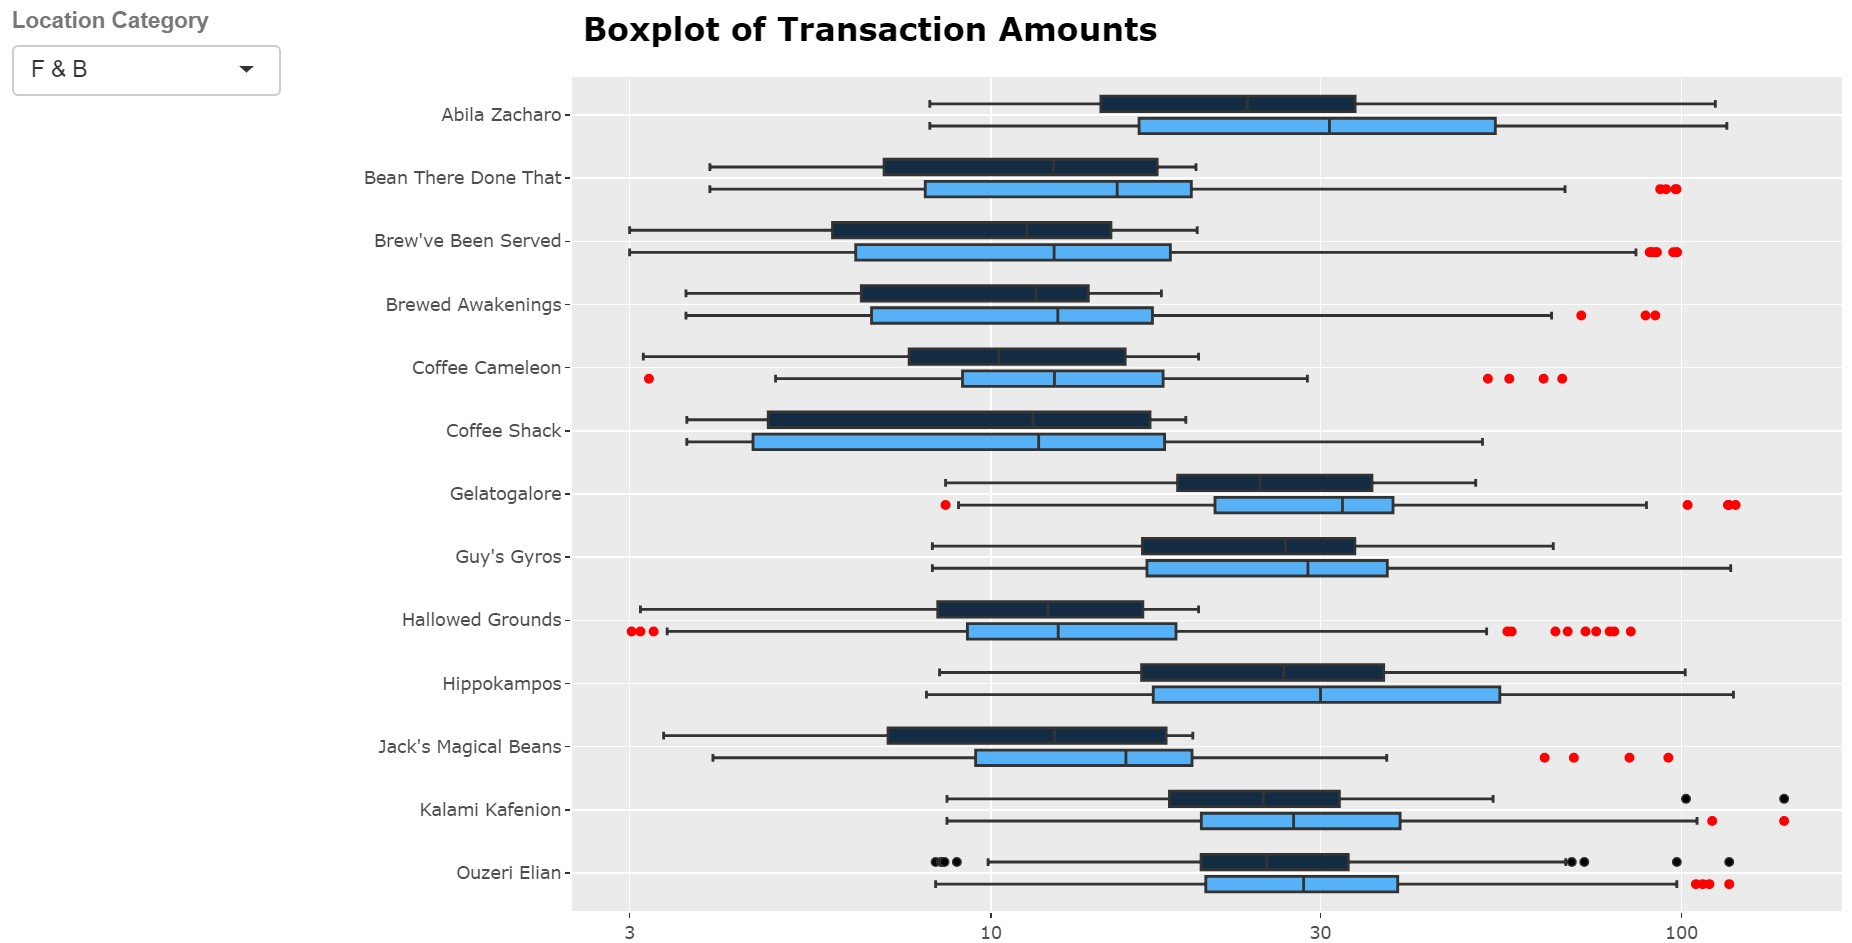
\includegraphics{img/P03BoxPlot.jpg} The plots are categorized by the
location types, as we believe transaction amounts should be compared
with those made at similar locations (For e.g.~F\&B with F\&B,
Industrial with Industrial). It would not be logical to compare a
transaction made at a supermarket, with one made at a chemical
production factory. This would be useful if the investigator wishes to
understand what is a normal range of transaction price for each
location, and which transactions deviated from the normal ranges. An
additional value-added feature that can be derived from this plot, is
the investigator can identify credit card and loyalty card pairs as they
would have the same transaction price, on the same day.

A further deep dive can be performed with the specific card transactions
scatter plot positioned below the overall boxplot.

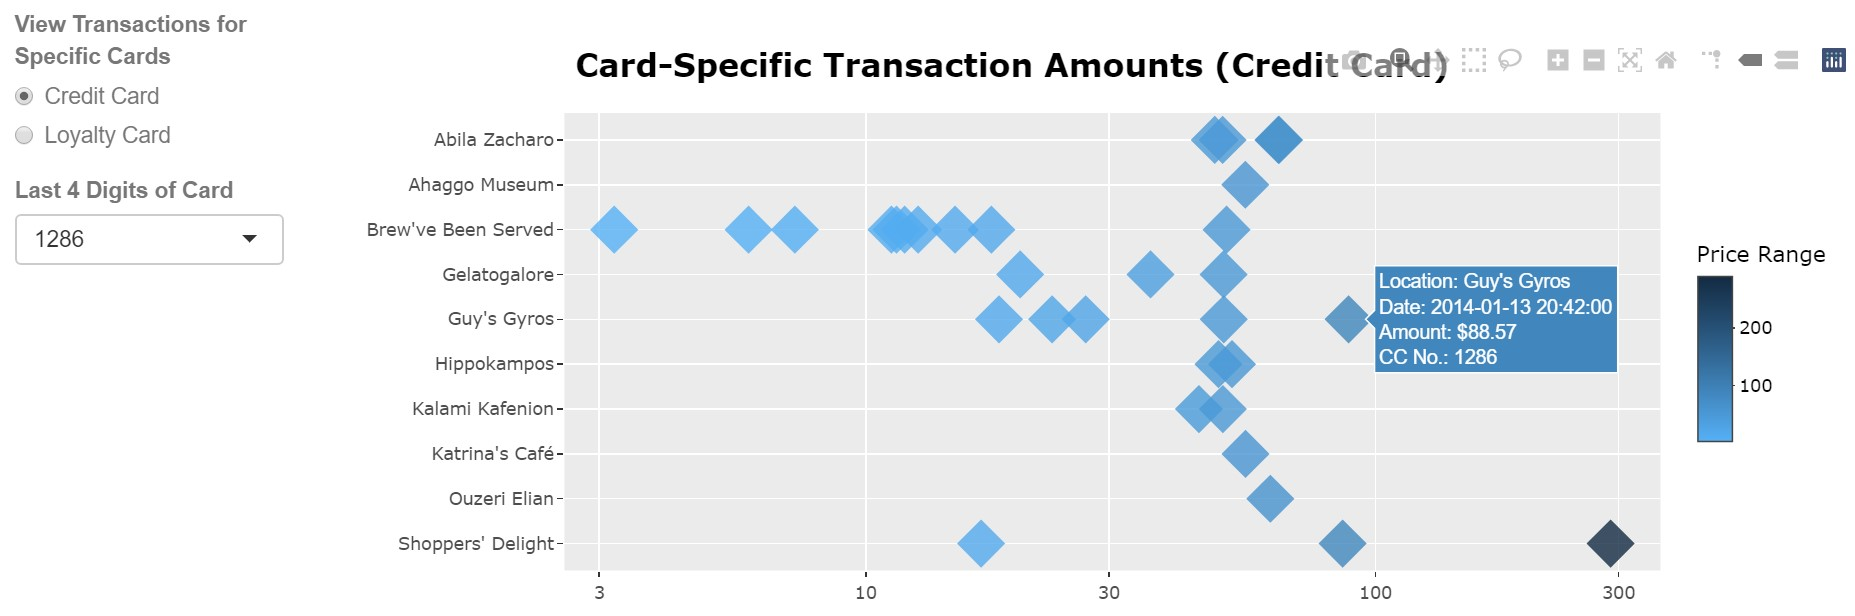
\includegraphics{img/P04SpecCardTxn.jpg}

This is a scatter plot of all transactions made by the card selected by
the investigator. Each point represents one transaction, and positioned
according to the transaction amount. How the amounts made at the same
location are relative to each other can be seen by their colors as well
- the darker the intensity, the higher the amount. As it is possible to
have multiple points clustered close together, some transparency is set
so that any overlaps are clearly visible.

\hypertarget{future-works}{%
\section{Future Works}\label{future-works}}

For the email network analysis, the data did not provide us with the
actual content of the email. While subjects can be useful for the
investigator to make reasonable judgments, there could be confirmation
biases and logical fallacies with that for e.g.~suspected members of the
POK using similar subjects for different email content.

This can be addressed with the provision of the email content data. In
addition to that, the text network can become more accurately with
better data.

The parallel coordinate plot in the Transactions Analysis Overview page
is currently only based on pure transactions data. Further insights
could be drawn, if the plot could be joined with data on vehicle IDs
which made stops at that particular location, in that particular period.
This would allow the investigator to narrow down which are the possible
vehicle IDs that could have made the transaction, or owned the credit
card/loyalty card. Linking to vehicle ID would enable the investigator
to link to the personnel based on who the vehicle is assigned to.

An improvement towards the Employee Movement Plot could include further
analysis on the movement route, in terms of the distance/ speed, which
may suggest the vehicle were kept in idle mode, which is currently
unable to detected under the current module. In addition, the streets of
Abila could be identified based on the movement routes, and thus, and
analysis could be conducted whether the vehicle was travelling in a
suspicious manner.

\hypertarget{acknowledgements}{%
\section{Acknowledgements}\label{acknowledgements}}

The authors wish to thank Professor Kam Tin Seong of Singapore
Management University for his extensive guidance and support during this
project.

\hypertarget{references}{%
\section{References}\label{references}}

\begin{longtable}[]{@{}
  >{\raggedright\arraybackslash}p{(\columnwidth - 0\tabcolsep) * \real{0.06}}@{}}
\toprule
\endhead
references: - id: IIITH title: VAST Challenge 2014 Mini Challenge 2
author: ``Pochampally, Yashaswi; Yarrabelly, Navya; Chikka, Veera
Raghavendra and Karlapalem, Karlapalem'' container-title:
`\url{http://visualdata.wustl.edu/varepository/VAST\%20Challenge\%202014/challenges/MC2\%20-\%20Patterns\%20of\%20Life\%20Analysis/entries/International\%20Institute\%20of\%20Information\%20Technology\%20Hyderabad/}'
URL:
`\url{http://visualdata.wustl.edu/varepository/VAST\%20Challenge\%202014/challenges/MC2\%20-\%20Patterns\%20of\%20Life\%20Analysis/entries/International\%20Institute\%20of\%20Information\%20Technology\%20Hyderabad/}'
type: website issued: year: 2014 \\
- id: UC title: VAST Challenge 2014 Mini Challenge 2 author: ``Sahaf,
Zahra et al.'' container-title:
`\url{http://visualdata.wustl.edu/varepository/VAST\%20Challenge\%202014/challenges/MC2\%20-\%20Patterns\%20of\%20Life\%20Analysis/entries/University\%20of\%20Calgary/}'
URL:
`\url{http://visualdata.wustl.edu/varepository/VAST\%20Challenge\%202014/challenges/MC2\%20-\%20Patterns\%20of\%20Life\%20Analysis/entries/University\%20of\%20Calgary/}'
type: website issued: year: 2014 \\
- id: profkam title: ``Hands-On Exercise 8: Creating Parallel Coordinate
Plot'' author: ``Kam, Tin Seong'' container-title:
`\url{https://rpubs.com/tskam/PCP}' URL:
`\url{https://rpubs.com/tskam/PCP}' type: website issued: year: 2020
month: 03 day: 13
\textless\textless\textless\textless\textless\textless\textless{}
HEAD \\
======= \\
- id: IIITH title: VAST Challenge 2014 Mini Challenge 1 author: ``Avil,
Pilar; Burgos, Valeria; Chikka, Guaymás Amalia'' container-title:
`\url{https://www.cs.umd.edu/hcil/varepository/VAST\%20Challenge\%202014/challenges/MC1\%20-\%20Disappearance\%20at\%20GASTech/entries/University\%20of\%20Buenos\%20Aires\%20-\%20Avila/}'
URL:
`\url{https://www.cs.umd.edu/hcil/varepository/VAST\%20Challenge\%202014/challenges/MC1\%20-\%20Disappearance\%20at\%20GASTech/entries/University\%20of\%20Buenos\%20Aires\%20-\%20Avila/}'
type: website issued: year: 2014 \\
- id: IIITH title: VAST Challenge 2014 Mini Challenge 1 author:
``Zhuang, Cai; Mengyao Chen;, Hanqing Zhao; Ying Zhao; Fangfang Zhou;
Kang Zhang;'' container-title:
`\url{https://www.cs.umd.edu/hcil/varepository/VAST\%20Challenge\%202014/challenges/MC1\%20-\%20Disappearance\%20at\%20GASTech/entries/Tianjin\%20University\%20-\%20Cai/}'
URL:
`\url{https://www.cs.umd.edu/hcil/varepository/VAST\%20Challenge\%202014/challenges/MC1\%20-\%20Disappearance\%20at\%20GASTech/entries/Tianjin\%20University\%20-\%20Cai/}'
type: website issued: year: 2014
\textgreater\textgreater\textgreater\textgreater\textgreater\textgreater\textgreater{}
parent of 86ead62 (adjust reference) \\
\bottomrule
\end{longtable}
\setlength{\parindent}{0in}

\end{document}
